\chapter{Results}
\label{chapter:Results}

The final output of this work is twofold.
\begin{itemize}
    \item{The first part presents an evaluation of support vector machines and ensemble learning methods under the domain of text classification methods. The particular problem being solved, as mentiond previously, is finding out the level of emotional distress amongst the general public, and finding out particular instances of the same. The distinguishing factor here is that the training data is not readily available, but is instead synthesized by tapping into crowd intelligence.}
    \item{The second part presents a web based interface, which is an implementation of these techniques and provides a system which can monitor the public feed from the Internet to find out people who are suffering emotional distress and may need help.}
\end{itemize}

\section{Evaluation}
\subsection{SVM}
SVMs (using linear, polynomial, radial basis, and sigmoid kernels) are evaluated.

Plot number of instances against -
\begin{itemize}
    \item{accuracy}
    \item{number of suppor vectors}
\end{itemize}

Scores [0.78436657681940702, 0.77789757412398919, 0.78490566037735854, 0.79083557951482475, 0.79299191374663069]

Mean 0.786199460916

\subsection{Ensemble Learning}
Ensemble learning methods are evaluated.

Plot number of instances against -
\begin{itemize}
    \item{accuracy}
\end{itemize}

Plot accuracy against -
\begin{itemize}
    \item{number of models in the ensemble}
    \item{sample weights (MATLAB plots from Han's implementation)}
\end{itemize}

\subsubsection{Bagging}
results from bagging

Scores [0.77789757412398919, 0.77196765498652287, 0.77681940700808627, 0.78490566037735854, 0.783288409703504]

Mean 0.77897574124

\subsubsection{Boosting}
results from boosting

Scores [0.65714285714285714, 0.65229110512129385, 0.66630727762803232, 0.65929919137466308, 0.660377358490566]

Mean 0.659083557951

\subsubsection{Stacking}
results from stacking

Scores [0.73153638814016175, 0.76442048517520211, 0.74231805929919137, 0.75202156334231807, 0.74555256064690023]

Mean 0.747169811321

\section{System Details}

The second major contribution of this thesis is a web based system that allows users to perform (broadly) the following functions - help build the training data, evaluate a level of distress amongst the general public, and find out particular people who have been posting content that appears to be distressed and qualifies as needing-attention.

Specifically, users can assign labels to stories fetched from reddit, which helps in building training data while tapping into crowd intelligence. The \emph{monitoring} module then presents information about a general level of distress amongst people who are posting on Twitter (grouped by date), and about certain tweets that have been classified as depressed. Showing information about particular tweets which have been classified as depressed presents authors of the tweet which may need further attention in the form of psychological help.

The system is divided into two modules - \emph{Ratings} and \emph{Monitoring}. This choice is presented to a user as soon as they visit the front page of the web interface, as shown in Figure~\ref{landing}.
\begin{figure}
    \centering
        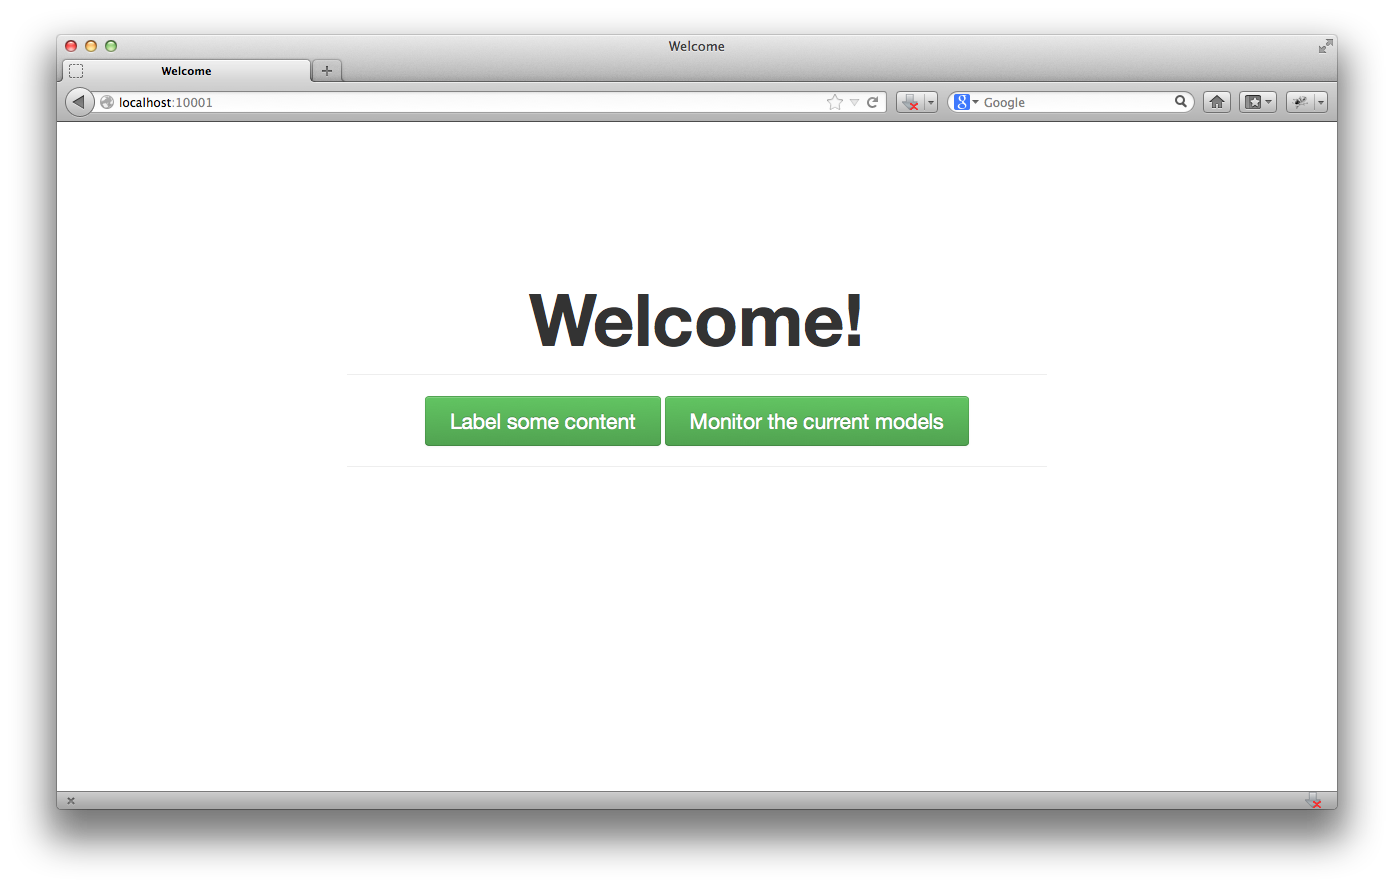
\includegraphics[width=\textwidth,scale=0.5]{landing.png}
    \caption{Landing page} \label{landing}
\end{figure}

The flow of the entire system can be seen as being divided into two parts. The first part, which is more manual, includes users fetching stories (from reddit) and labelling them, which helps in building the training data. The second part is built using automatic cron jobs (pieces of code that are executed after specific intervals of time), and involves the following -
\begin{itemize}
    \item{every 3 hours - fetching 100 tweets from the public stream of Twitter}
    \item{every morning - assigning labels to all tweets fetched from Twitter according to the updated model}
\end{itemize}

\section{Ratings}
The \emph{Ratings} module is built to help consolidate the training data. Users are provided with options to label the unlabeled data (as ``depressed'' or ``not depressed'') that is already present in the database. If in case there are no unlabeled stories left, then there also exists an option to fetch more data from Reddit. When invoked, this option fetches 500 stories each from \href{http://www.reddit.com/r/happy}{/r/happy} and \href{http://www.reddit.com/r/suicidewatch}{/r/suicidewatch}.

As shown in Figure~\ref{ratings}, the user is presented with a random piece of text that was fetched from Reddit, and two buttons for assigning this story a label.

\begin{figure}
    \centering
        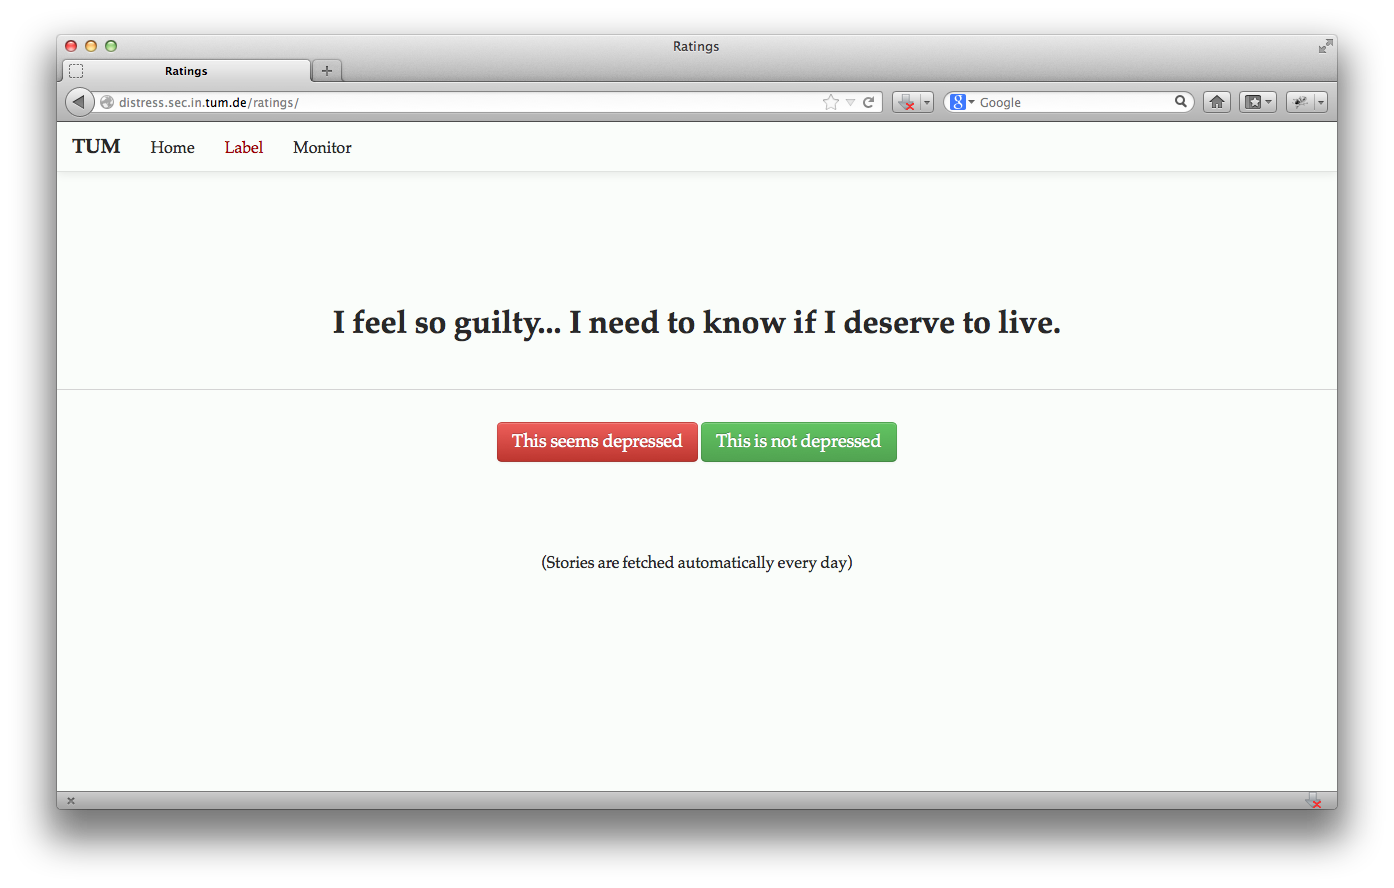
\includegraphics[width=\textwidth,scale=0.5]{ratings.png}
    \caption{Ratings module} \label{ratings}
\end{figure}

\section{Monitoring}
